\section{引言}

\eng{LWIR} 热成像通过测量缺陷与工艺偏差引起的亚摄氏度温度差异，已成为半导体无损检测的关键手段
\cite{breitenstein2010lockin}。在这类应用中，检测结论直接基于重建图像判读，重建中引入的虚假结构
特征将导致误判，而非仅仅带来模糊。然而该成像模态同时受到物理与数据条件的约束：光学系统受衍射限制，
截止频率以上的空间结构无法被传递；更高端的光学方案成本高昂且增益有限；而学习类超分辨所依赖的
高分辨率热成像配对真值也不可获得。因此，核心问题是：能否以多帧计算增强替代硬件升级，让这些轮廓在现有仪器上可靠地更加清晰。

微扫描为此提供了物理基础。电动台以亚像素步长平移场景并逐帧采集，使序列携带了单帧不具备的
亚像素相位多样性，构成经典多帧超分辨的标准设定 \cite{tsai1984multiframe,farsiu2004fast}。
然而这一设定伴随一个根本性的困难：在整个采集与部署过程中，始终不存在高分辨率热成像真值。
在该模态与该场景下不存在配对的 \eng{HR} 传感器，光学显微在辐射学上不可比且未与热成像配准。
由此，学习类 \eng{SR} 所依赖的配对训练数据、全参考评估指标以及基于验证 \eng{PSNR} 的模型选择，
在真实数据上全部失效。

\begin{figure}[t]
  \centering
  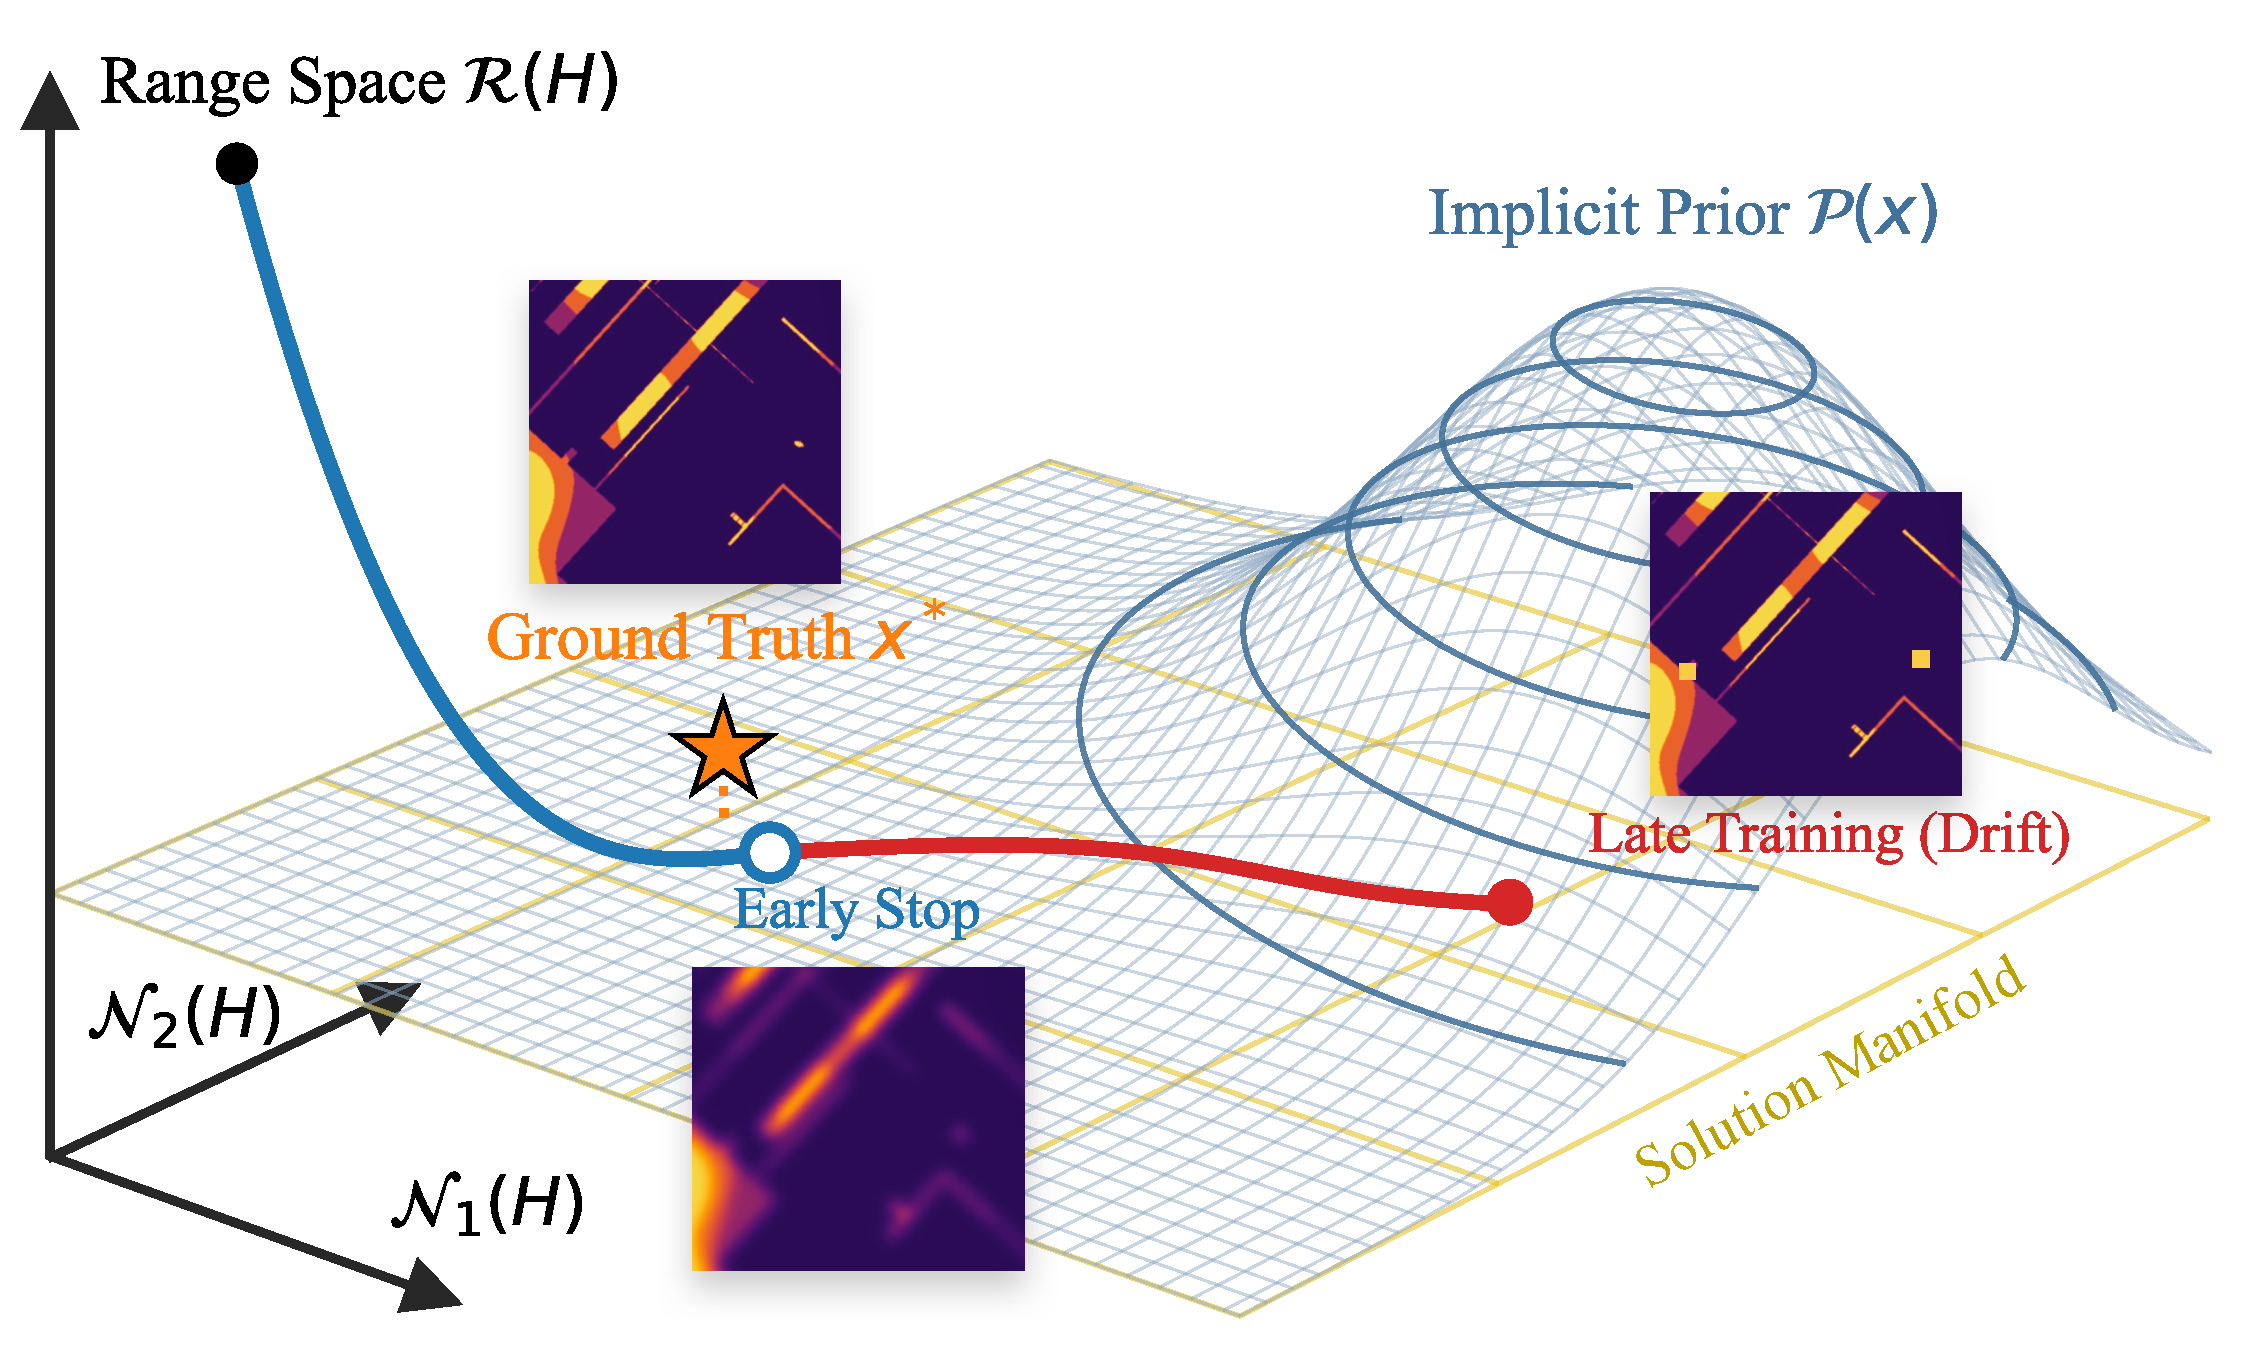
\includegraphics[width=0.95\linewidth]{../figures/fig_nullspace_drif.pdf}
  \caption{零空间漂移示意图。纵轴为值域 $\mathcal{R}(H)$，水平面为零空间张成的解流形。流形上所有解产生相同的低分辨率观测，因而观测侧损失无法区分。训练先沿值域方向下降至流形（蓝色曲线），此后沿零空间向隐式先验 $\mathcal{P}(x)$ 漂移（红色路径），远离真值 $x^*$。嵌入热图示意：早停解与晚期漂移解的观测一致性相近，重建结果却已显著不同。}
  \label{fig:teaser}
\end{figure}

在自然图像超分辨等领域，应对无配对真值的常见策略是在合成退化数据上训练后
直接部署到目标域，并以表观细节更丰富的输出作为改进证据
\cite{wang2021real,zhang2021designing}。然而在无真值场景下，
“看起来细节更多”恰是失效模式而非成功标志 \cite{mittal2013making}。这一风险通常被称为
幻觉，在社区中已被广泛认识，但很少被系统地量化。本文的目标是量化这一现象、
刻画其产生机制，并构建一套能在定量检验下存活的 \(2\times\) 轮廓级增强管线。

我们围绕三个递进的问题组织全文。第一，信息是否存在：多帧观测序列中是否确实含有超出单帧分辨率的
可恢复信息。我们通过带正、负、漂移控制组的相位分层分半 \eng{FRC} \cite{vanheel2005fourier}
为多帧序列的相干信息量定界，并以经典去卷积基准将这一余量兑现为所有学习类方法必须达到的基线门槛。
第二，信息是否送达：学习类方法是否真正接收到了亚像素相位信息。固定网络架构与损失函数、
仅替换输入表示的对比实验表明，在常规逐帧统计特征输入下，亚像素相位在输入编码阶段即已坍塌，
网络无法利用；只有将同一信息以更细网格的 drizzle 通道注入后，相位结构才在训练中可见。第三，细节是否忠实：模型新增的细节是否锚定于观测。这是本文的核心发现——如图~\ref{fig:teaser}~所示，合成训练的网络在真实数据上沿观测算子的零空间漂移
\cite{schwab2019deep,chen2021equivariant}：前向一致性损失停在噪声底部，而真实数据上的
伪影诊断持续劣化，任何有界的观测域锚定项均对该漂移分量不可见。有效的补救不在于更强的一致性惩罚，
而在于输入侧的证据注入与机械化的选点规则。

\textbf{贡献.}\ 
(1)~揭示并刻画了无真值热成像多帧超分辨中的\zhemph{零空间漂移}现象：在物理匹配的合成数据上训练的网络迁移至真实数据后，诊断证据显示其新增高频细节与观测算子的零/近零空间漂移一致；结合固定观测算子的零/近零空间分析（附录 A.2），任何有界的观测侧锚定项对这一漂移分量均不可见，因此有效补救在于输入侧的证据注入——以更细网格的 drizzle 通道把亚像素相位重新送入网络。
(2)~在一套无高分辨率真值的评估协议下给出经典 vs.\ 学习类的诚实裁决：该协议以相位分层分半 \eng{FRC}（带正/负/漂移控制组）为多帧序列的相干信息量定界，并辅以一对观测锚定代理指标与机械化的检查点选点规则（详见附录 A.3--A.4、C.5），其本身只能提供有界的、代理级别的判据，而非光学真值。在此判据下，经典变分重建在可验证的观测指标上最为保真，学习类重建表观细节最多但携带最多不可验证的高频内容，二者呈现互补的失效模式；正因为可用的判据是有界的，在缺乏高分辨率热真值的条件下，不存在可认证的单一最优方法。
